%----------------------------------------------------------------------------------------
%	PACKAGES AND THEMES
%----------------------------------------------------------------------------------------
\documentclass{beamer}
% Load a bunch of useful packages:
\usepackage{amssymb,amsmath,amsfonts,mathtools} % useful math fonts and symbols
\usepackage{geometry} % allows changing margins and sizes of stuff
\usepackage{hyperref} % allows referencing of lines of text, urls, figures etc
\usepackage{natbib} % allows citation referencing from a .bib file
\bibliographystyle{apalike} % American Psychological Association style guide
\usepackage{graphicx} % to include graphics from the figures folder with helpful formating options
\usepackage{tikz}
\usetikzlibrary{arrows}
\usepackage{pgfplots}
\usetikzlibrary{calc}
%---------------------------------------------%
\usepackage{color} % custom color definitions:%
    %UOregon colors:                          %
    \definecolor{UOGreen}{RGB}{18, 71, 52}    %
    \definecolor{UOYellow}{RGB}{254, 225, 35} %
    %Secondary official colors:               %
    \definecolor{LegacyGreen}{HTML}{104735}   %
    \definecolor{GrassGreen}{HTML}{489D46}    %
    \definecolor{LimeGreen}{HTML}{8ABB40}     %
    \definecolor{Chartreuse}{HTML}{E2E11B}    %
    \definecolor{Berry}{HTML}{8D1D58}         %
    \definecolor{DarkBlue}{HTML}{004F6E}      %
    \definecolor{LightBlue}{HTML}{00A5B5}     %
    \definecolor{crimson}{RGB}{ 170, 4, 36 }
    \definecolor{darkblue}{RGB}{ 4, 47, 170 }
    \definecolor{brown}{RGB}{ 111, 71, 2 }
    \definecolor{periwinkle}{RGB}{ 90, 177, 204 }
    \definecolor{ducksgreen}{HTML}{007030}
%----------------------------------------------

\usepackage{setspace} % to specify single, double or one-half spacing of text
\usepackage{indentfirst} % indent first line of a text paragraph
\usepackage{multicol} %multipage ability
\usepackage{multirow}
\usepackage{ulem} % \ul (underline) command which will break over line ends
\usepackage{amsthm} % allows standarized theorem commands
\setbeamertemplate{theorems}[numbered]
\theoremstyle{plain}
\newtheorem{assume}{Assumption}
\newtheorem{define}{Definition}
\usepackage{breqn} %automatic line breaking
\usepackage{enumitem}
\setitemize{label=\usebeamerfont*{itemize item}%
  \usebeamercolor[fg]{itemize item}
  \usebeamertemplate{itemize item}}
\normalem
\usepackage{array}

% Theming and Appearance Setup:
\usetheme{metropolis}
\metroset{block=fill}
%\usetheme{default}
\usefonttheme{professionalfonts}
\fontfamily{ppl}\selectfont
\usecolortheme[named=UOGreen]{structure}
\setbeamertemplate{footline}[frame number]
\setbeamertemplate{headline}{} %Removes Section Index on top of slide
\beamertemplatenavigationsymbolsempty
\hypersetup{
    colorlinks=true,
    linkcolor=DarkBlue,
    filecolor=Berry,
    citecolor=GrassGreen,
    urlcolor={LightBlue},
    pdftitle={Trade and Labor Market Dynamics},
    pdfpagemode=FullScreen
}

%------------------------------------------------------------------------------%TITLE PAGE
%------------------------------------------------------------------------------
% The title
\title{Repeated Games}
\author{Dante Yasui }
\institute{EC327 Game Theory}
\date{Fall 2025}
\titlegraphic{\includegraphics[scale=.4]{UOSignature-356.png}}


%-----------------------------------------------------------------------------
%	PRESENTATION SLIDES
%-----------------------------------------------------------------------------

\begin{document}

\begin{frame}[plain]
    % Print the title page as the first slide
    \titlepage
\end{frame}
\addtocounter{framenumber}{-1}

% \begin{frame}[plain]{Outline}
%   \tableofcontents
% \end{frame}
% \addtocounter{framenumber}{-1}

% - - - - - - - - - - - - - - - - - - - - - - - - - - - - - - - - - - - - - -


\begin{frame}{}
  \begin{itemize}
    \item So far, games either \textbf{one-shot} simultaneous or \textbf{finitely sequential}
    \item However, how to represent situations in which \textbf{repeated interactions} matter?
    \begin{itemize}
      \item how do \alert{reputation}, \alert{shared history}, etc matter for strategy?
      \item power of \alert{institutions} to coordinate cooperation
    \end{itemize}
  \end{itemize} 
\end{frame}

\begin{frame}
  What do we mean by \textit{cooperative} behavior?
  \begin{itemize}
    \item \textit{altruism}
    \begin{itemize}
      \item cooperation that ignores self-interest
    \end{itemize}
    \item \textbf{\alert{cooperation}}
    \begin{itemize}
      \item cooperation achieved through self-interest
      \item rational self-interest may still lead to pro-social behavior
      \item more robust policy design to assume everyone is self-interested
      (but will respond to incentives)
      than to try to rely on pure altruism
    \end{itemize}
  \end{itemize}
\end{frame}

\begin{frame}
  \frametitle{Repeated Games Framework}
  A \alert{repeated game} is one with potentially infinte subgames
  \begin{itemize}
    \item payoffs are realised in each stage
    \item each \textit{stage} subgame is identical and itself is a \textit{regular} subgame
    \item \alert{perfect recall} - common knowledge of shared history
    \begin{itemize}
      \item strategies may be contingent on observed history
    \end{itemize}
    \item stage subgame is either repeated \textit{infinitely} or \textit{probabalistically}
  \end{itemize}
  \begin{itemize}
    \item infinite strategies are complicated, so we need \alert{present value} calculations
  \end{itemize}
\end{frame}

\section*{Trench Warfare as Repeated Prisonners' Dilemma}
% Section 1: Trench Warfare in WWI
%---------------------------------------------------------------------------

\begin{frame}{Trench Warfare in WWI}
  \begin{itemize}
    \item On the Western Front, 
    early advances ground to a halt and stagnated into trench warfare
    \item Technologies like artillery and machine guns made the war one of the bloodiest in human history
  \end{itemize}
\end{frame}

\begin{frame}{Trench Warfare in WWI}
  \begin{center}
  \includegraphics[width=1\textwidth]{figures/fig131.png}
  \end{center}
  What's the \textbf{NE}?
\end{frame}

\begin{frame}{Unexpected Truces Emerge}
  Christmas Day Truce, 1914:
  \begin{center}
    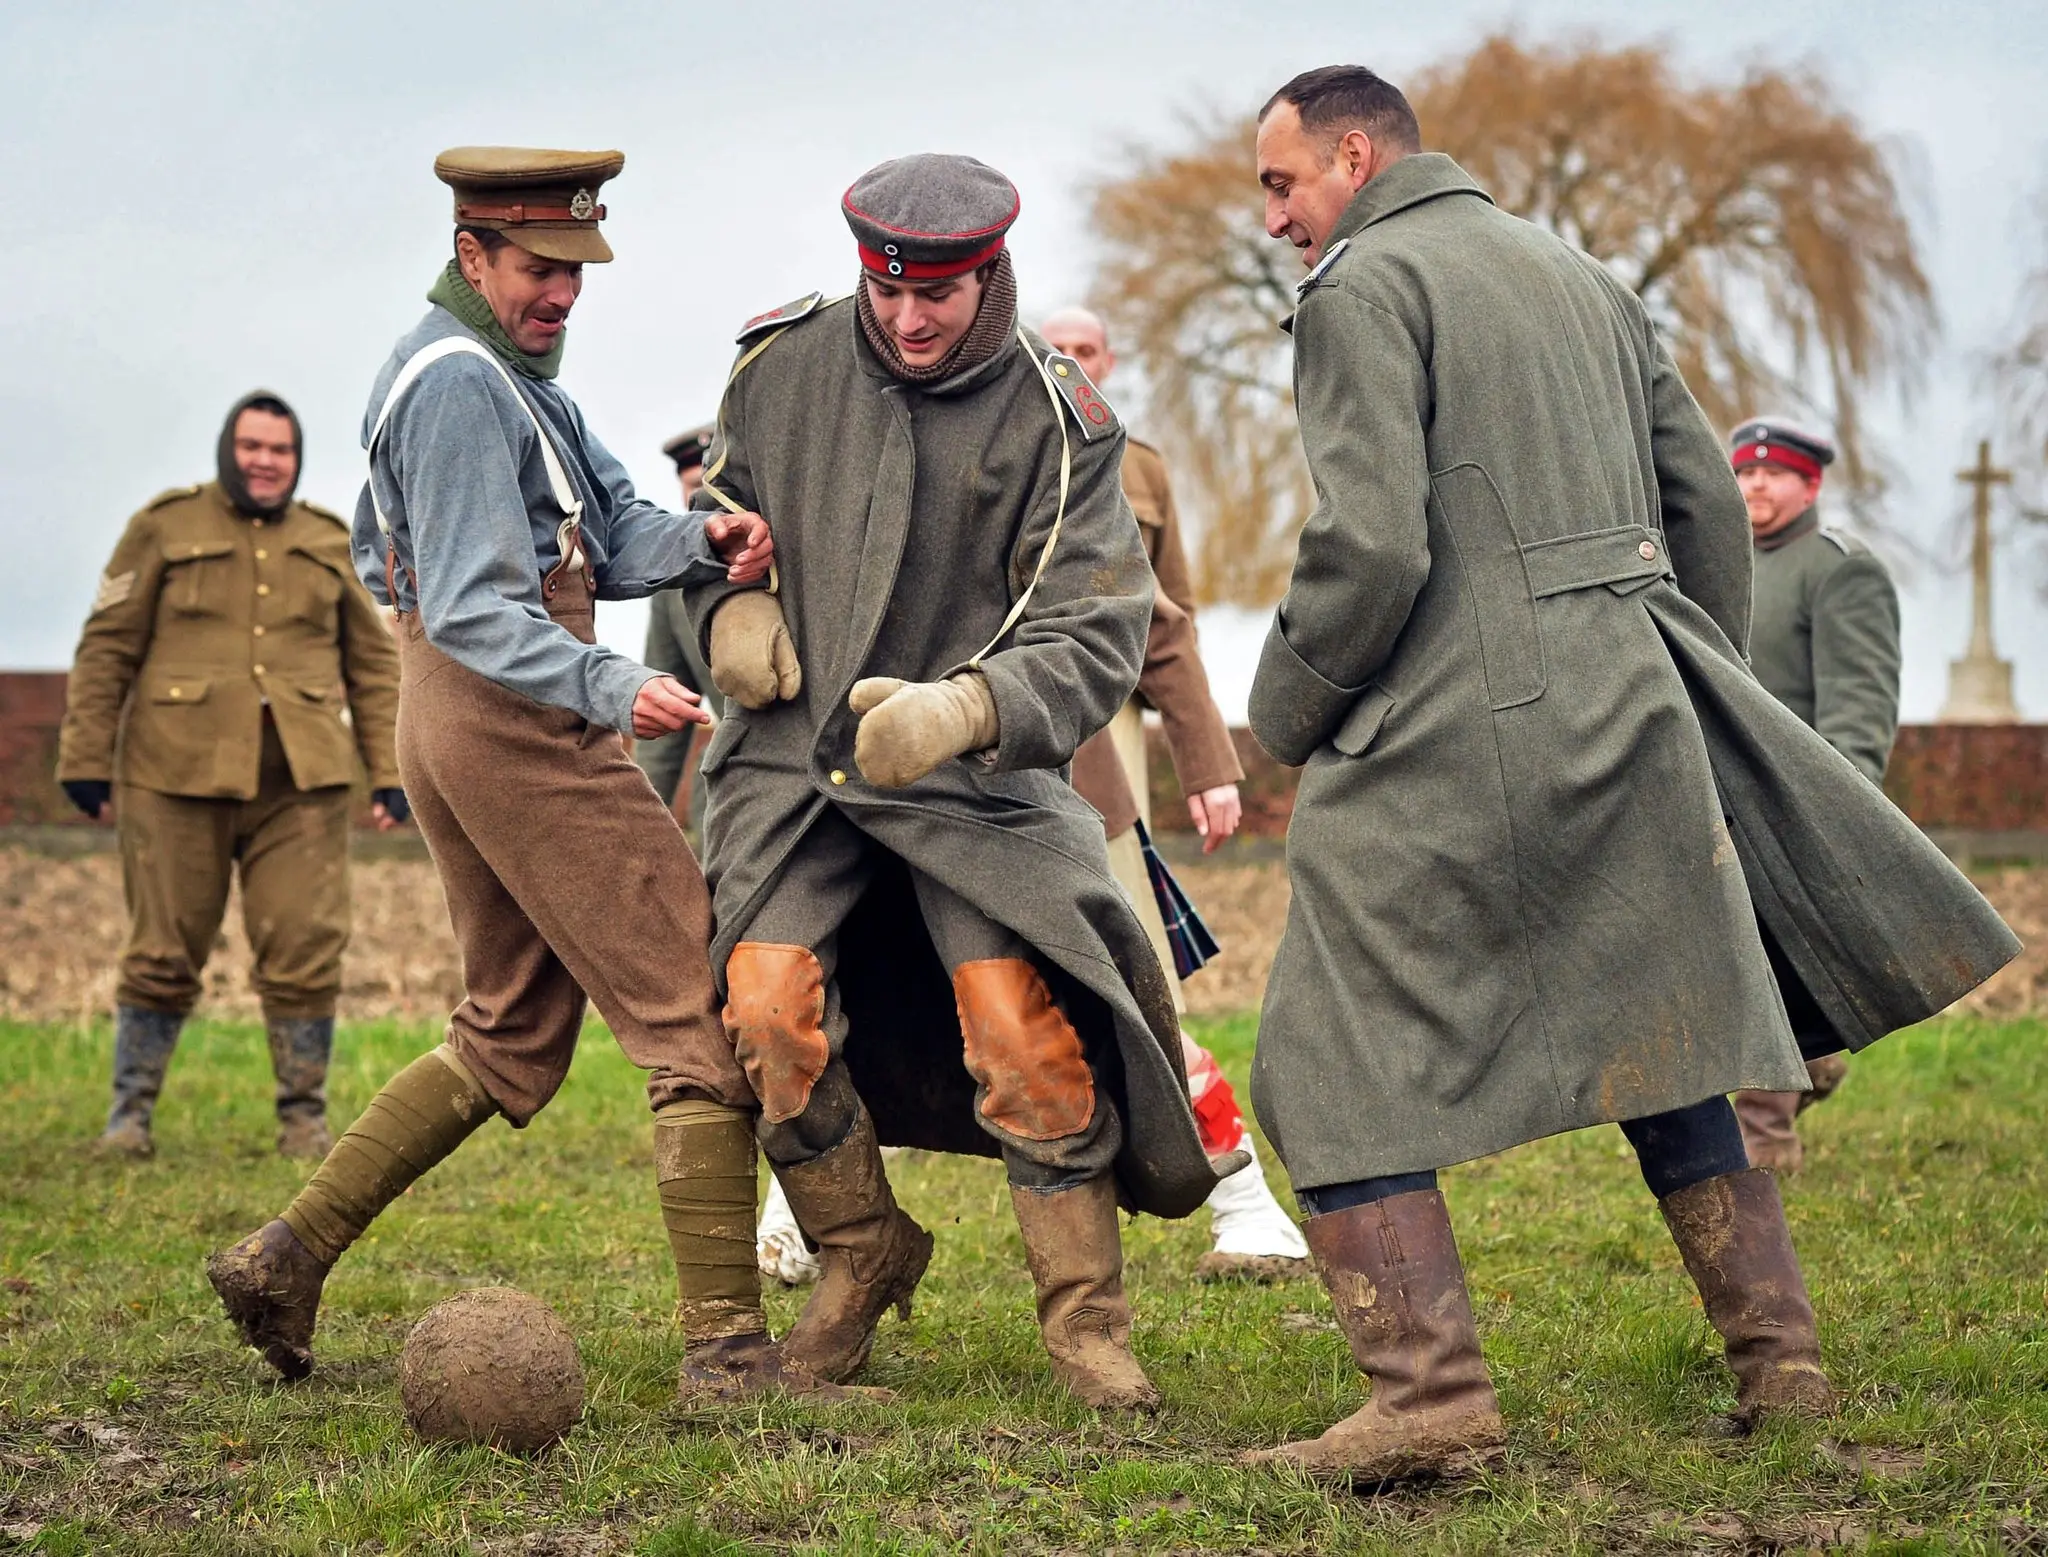
\includegraphics[width=.75\textwidth]{figures/hughes24-superJumbo.png} 
  \end{center}
  {\footnotesize Image Credit: Stephanie Lecocq/European Pressphoto Agency}
\end{frame}

\begin{frame}{Unexpected Truces Emerge}
  \begin{quote}
    \footnotesize 

    So regular were [the Germans] in their choice of targets, times of shooting, and number of rounds fired, that, after being in the line one or two days, Colonel Jones had discovered their system, and knew to a minute where the next shell would fall. His calculations were very accurate, and he was able to take what seemed to uninitiated Staff Officers big risks, knowing that the shelling would stop before he reached the place being shelled.

    I was having tea with A Company when we heard a lot of shouting and went out to investigate. We found our men and the Germans standing on their respective parapets. Suddenly a salvo arrived but did no damage. Naturally both sides got down and our men started swearing at the Germans, when all at once a brave German got on to his parapet and shouted out “We are very sorry about that; we hope no one was hurt. It is not our fault, it is that damned Prussian artillery.”
  \end{quote} 
\end{frame}

\begin{frame}{The puzzle of trench truces}
  \begin{itemize}
    \item How did cooperation between enemy armies achieved and sustained?
    \item One answer might be that in these parts of the front, interactions were \textbf{repeated} between the same units
  \end{itemize} 
\end{frame}

\begin{frame}{Constructing a Repeated Game}
  \begin{itemize}
    \item Suppose that Allied and German forces anticipate that they will play this game $T$ times 
  \end{itemize}
  \begin{center}
    \includegraphics[width=.5\textwidth]{figures/fig131.png}  
  \end{center}
  \begin{itemize}
    \item A \textit{strategy} will be made up of $T$ \textit{actions}; 
    one for each time this stage game is played
  \end{itemize}
\end{frame}

% \begin{frame}{Constructing a Repeated Game}
%   To represent this as an extensive form tree, lets suppose that $T=2$:
%   \begin{itemize}
%     \item If neither side sees what their opponent's strategy was yesterday, each player has 3 info sets
%     \item So each side has eight possible strategies:
%     \begin{itemize}
%       \item (\textit{Kill$_1$}, \textit{Kill$_2$} if \textit{Kill$_1$} or \textit{Miss$_1$})
%       \item (\textit{Kill$_1$}, \textit{Kill$_2$} if \textit{Kill$_1$} else \textit{Miss$_2$} if \textit{Miss$_1$})
%       \item (\textit{Kill$_1$}, \textit{Miss$_2$} if \textit{Kill$_1$} else \textit{Kill$_2$} if \textit{Miss$_1$})
%       \item (\textit{Kill$_1$}, \textit{Miss$_2$} if \textit{Kill$_1$} or \textit{Miss$_1$})
%       \item ...
%     \end{itemize}
%   \end{itemize}
% \end{frame}

% \begin{frame}{Constructing a Repeated Game}
%   \begin{center}
%     \includegraphics[width=1\textwidth]{figures/fig132.png} 
%   \end{center} 
% \end{frame}

\begin{frame}{Constructing a Repeated Game}
  To represent this as an extensive form tree, lets suppose that $T=2$:
  and suppose that the history of all past plays are \textbf{common knowledge} 
  \begin{itemize}
    \item each player will have five info sets; one for day 1, and four in day 2 
    \item What does the extensive form game look like?
  \end{itemize}
\end{frame}

\begin{frame}{Constructing a Repeated Game}
  \begin{center}
    \includegraphics[width=1\textwidth]{figures/fig133.png} 
  \end{center} 
\end{frame}

\begin{frame}{Constructing a Repeated Game}
  Let's generalize what a strategy in \textit{any} \alert{finitely repeated game} with \alert{common knowledge} will look like:
  \begin{itemize}
    \item If a game has $T$ periods, and each player has $m$ actions at each stage,
    \item there is one initial info set, $m^2$ info sets in period 2, $m^4$ info sets in period 3, ..., $m^{2(T-1)}$ in the last period 
    \item A complete strategy is made up of $1 + m^2 + m^4 + ... + m^{2(T-1)}$ actions 
  \end{itemize}
  In an \alert{infinitely repeated game}, there will be an infinite number of actions in each strategy
\end{frame}

\begin{frame}{Constructing a Repeated Game}
  How to model streams payoffs over time?
  \begin{itemize}
    \item We could just add up all of the per-stage payoffs across an entire history
    \item But for infinitely-long histories, this sum would blow up and not make much sense
    \item Instead, we will use \alert{present value} calculations
  \end{itemize}
\end{frame}

\begin{frame}{Present Values}
  Suppose that I have an income stream where I earn $w_t$ dollars in every year $t$
  \begin{itemize}
    \item Suppose that there is a single \alert{discount factor} $\delta$ which captures how much I value income tomorrow compared to income today
    \item My present value over my whole income stream is 
    $$ w_1 + \delta w_2 + \delta^2 w_3 + \delta^3 w_4 + ... + \delta^{T-1} w_T $$
    \item It makes sense to assume that $0<\delta<1$ because I should probably care about tomorrow to some extent, but not as much as today
  \end{itemize}
\end{frame}

\begin{frame}{Present Values}
  What about calculating a present value of an \alert{infinte stream} of payoffs?
  \begin{itemize}
    \item It turns out:  
    $$ x + \delta x + \delta^2 x + \delta^3 x + ... + \delta^{\infty} x $$
    \item actually converges to $\frac{x}{1-\delta}$ as long as $\delta<1$ 
  \end{itemize}
\end{frame}

\begin{frame}{Check Your Understanding}
  Suppose you are deciding between three different payoff streams:
  \vspace{5mm}

  \begin{center}
  \begin{tabular}{|c|c|c|c|}
    \textbf{Period} & \textbf{Stream A} & \textbf{Stream B} & \textbf{Stream C} \\ \hline 
    1 & 15 & 25 &  5 \\ 
    2 & 15 & 15 & 10 \\ 
    3 & 15 & 10 & 20 \\ 
    4 & 15 &  5 & 30 \\
  \end{tabular}
  \end{center}

  \vspace{5mm}
  Which has the \textbf{highest present value} when $\delta =0.8$?
  \pause
  
  Stream A: 44.28, \textbf{Stream B: 45.9}, Stream C: 41.16
\end{frame}

\begin{frame}{Going back to the trenches}
  \begin{center}
    \includegraphics[width=.8\textwidth]{figures/fig133.png} 
  \end{center}  
  This was our extensive form game for only 2 periods
\end{frame}

\begin{frame}{Going back to the trenches}
  Now suppose that we have a potentially very large $T$

  How can we find a SPNE?

\end{frame}

\begin{frame}{Going back to the trenches}
  Suppose that we are already at the last period $T$ of the $T$-period trench warfare game 

  Suppose that the Allies total payoff stream value so far is $A^{T-1}$ and the Germans is $G^{T-1}$ 
  \begin{center}
    \includegraphics[width=.7\textwidth]{figures/tab137.png} 
  \end{center}
  What will happen?
  \pause

  \begin{itemize}
      \item Allies will Shoot to \textbf{Kill},
      Germans will Shoot to \textbf{Kill}
  \end{itemize}
\end{frame}

\begin{frame}{Going back to the trenches}
  Now that we know the $T$ stage will end in $(Kill, ~Kill)$, we can look one period back to what will happen in $T-1$: 
  \begin{center}
    \includegraphics[width=.7\textwidth]{figures/fig138.png}
  \end{center}
  What will happen?
  \pause
  \begin{itemize}
      \item Both will shoot to \textbf{Kill} in $T-1$, knowing they will both shoot to kill in $T$
  \end{itemize}
\end{frame}

\begin{frame}{Trench Game with Finite stages}
  By now, you should get the idea:
  \begin{block}{Insight}
    If the stage game has a unique NE, then any finitely repeated version will
    have a unique SPNE which is just the repetition of the single-stage NE. No
    cooperation is sustainable 
  \end{block}

  So what was going on with those spontaneous truces?
\end{frame}

\begin{frame}{Infinitely Repeated Trench Game}
  \begin{itemize}
    \item The problem with that last equilibrium we found was that you have to
      know \textit{exactly when the game will end} to use backwards induction 
    \item But for World War I infantrymen, they didn't know how long it would
      be until the fronts shifted or their division was rotated out
    \item We will have to extend our models to allow for 
      \alert{indefinite horizons}
  \end{itemize} 
\end{frame}

\begin{frame}{Repeated Prisoners' Dilemma with Uncertain Second Stage}
  Suppose that the first stage of the game is the Trenches Game:
  \begin{table}[!h]
    \centering
    \begin{tabular}{*{4}{c|}}
      \multicolumn{2}{c}{} & \multicolumn{2}{c}{German soldiers} \\ \cline{3-4}
      \multicolumn{1}{c}{} &    & Kill & Miss \\ \cline{2-4}
      \multirow{2}*{Allied Soldiers} & Kill & 4, 4 & 8, 2 \\ \cline{2-4}
                         & Miss & 2, 8 & 6, 6 \\ \cline{2-4} 
    \end{tabular} 
  \end{table}
  But with probability $p$, the game repeats in the second round 
  and with probability $1-p$, it ends after the first round
\end{frame}

\begin{frame}{Repeated Prisoners' Dilemma with Uncertain Second Stage}
  Consider the following strategy: 
  \begin{align*}
    \begin{cases}
      \text{In stage } 1 & : \textit{Miss} \\ 
      \text{In stage } 2 & : 
      \begin{cases}
        \textit{Miss} \text{  if the other player Missed in stage 1} \\ 
        \textit{Kill} \text{  if the other player Killed in stage 1}
      \end{cases}
    \end{cases}
  \end{align*}
  Let's call this strategy \textit{Punisher} because it starts off friendly, 
  but will try to punish someone who defects in the first round by defecting in the second round.
\end{frame}

\begin{frame}{Repeated Prisoners' Dilemma with Uncertain Second Stage}
  Suppose you are playing against a \textit{Punisher} in this game. 

  \begin{center}
    \begin{tabular}{*{4}{c|}}
      \multicolumn{2}{c}{} & \multicolumn{2}{c}{German soldiers} \\ \cline{3-4}
      \multicolumn{1}{c}{} &    & Kill & Miss \\ \cline{2-4}
      \multirow{2}*{Allied Soldiers} & Kill & 4, 4 & 8, 2 \\ \cline{2-4}
                         & Miss & 2, 8 & 6, 6 \\ \cline{2-4} 
    \end{tabular} 
  \end{center}

  \begin{itemize}
    \item What is your \textbf{expected utility} of playing \textit{Kill}, \textit{Kill}?
    \pause
    \item 8 in the first stage, 4 in the second stage,
    \item so $EU(Kill,~Kill) = 8 + 4p$
  \end{itemize}
\end{frame}

\begin{frame}{Repeated Prisoners' Dilemma with Uncertain Second Stage}
  Suppose you are playing against a \textit{Punisher} in this game. 

  \begin{center}
    \begin{tabular}{*{4}{c|}}
      \multicolumn{2}{c}{} & \multicolumn{2}{c}{German soldiers} \\ \cline{3-4}
      \multicolumn{1}{c}{} &    & Kill & Miss \\ \cline{2-4}
      \multirow{2}*{Allied Soldiers} & Kill & 4, 4 & 8, 2 \\ \cline{2-4}
                         & Miss & 2, 8 & 6, 6 \\ \cline{2-4} 
    \end{tabular} 
  \end{center}

  What is your \textbf{expected utility} of playing \textit{Miss, Kill}? \\
  \pause
  \begin{itemize}
      \item $4 + 8p$
  \end{itemize}
  What about from playing \textit{Kill, Miss?} \\
  \pause
  \begin{itemize}
      \item $8 + 2p$
  \end{itemize}
  Would you rather defect earlier or later?
\end{frame}

\begin{frame}{Repeated Prisoners' Dilemma with Uncertain Second Stage}
  Suppose you are playing against a \textit{Punisher} in this game. 

  \begin{center}
    \begin{tabular}{*{4}{c|}}
      \multicolumn{2}{c}{} & \multicolumn{2}{c}{German soldiers} \\ \cline{3-4}
      \multicolumn{1}{c}{} &    & Kill & Miss \\ \cline{2-4}
      \multirow{2}*{Allied Soldiers} & Kill & 4, 4 & 8, 2 \\ \cline{2-4}
                         & Miss & 2, 8 & 6, 6 \\ \cline{2-4} 
    \end{tabular} 
  \end{center}

  What is your \textbf{expected utility} of playing \textit{Miss, Miss}?
  \begin{itemize}
      \item $6 + 6p$
  \end{itemize}
\end{frame}

\begin{frame}{Repeated Prisoners' Dilemma with Uncertain Second Stage}
  Let's graph your expected utilties of each strategy:
  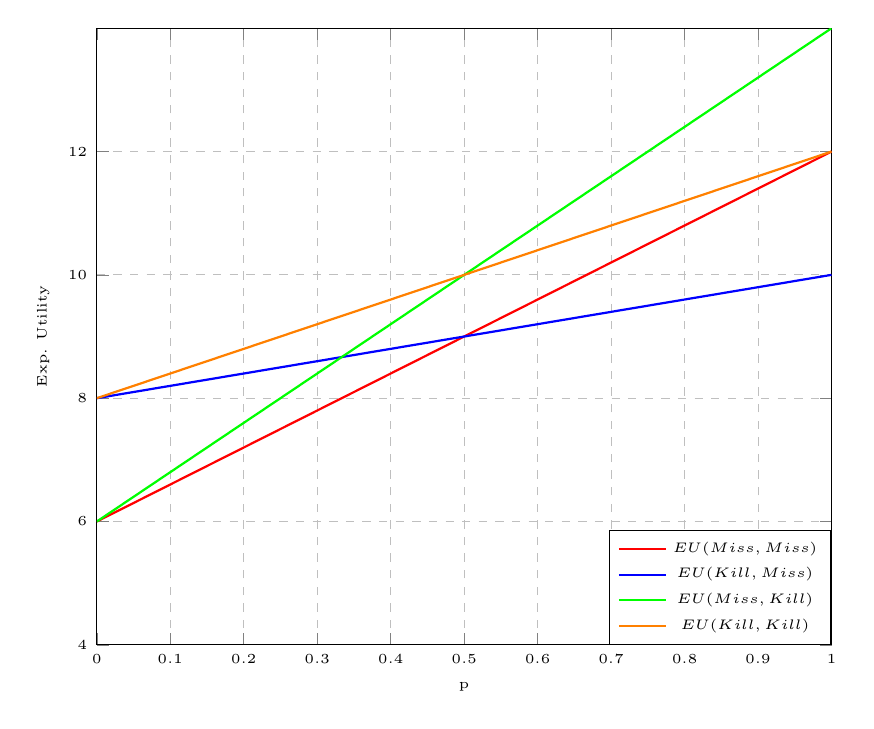
\begin{tikzpicture}
   \begin{axis}[
     width=0.9\textwidth,
     grid,
     xlabel={p},
     ylabel={Exp. Utility},
     xmin=0, xmax=1.0,
     ymin=4, ymax=14,
     xtick={0,.1,...,1.0},
     ytick={2, 4, 6, 8, 10, 12},
     grid style=dashed,
     font=\tiny,
     legend style={at={(1,0)},anchor=south east},
     ]
 
     \addplot[domain=0:1, samples=100, thick, red] {6 + 6*x};
     \addlegendentry{$EU(Miss, Miss)$}

     \addplot[domain=0:1, samples=100, thick, blue] {8 + 2*x};
     \addlegendentry{$EU(Kill, Miss)$}

     \addplot[domain=0:1, samples=100, thick, green] {6 + 8*x};
     \addlegendentry{$EU(Miss, Kill)$}
     
     \addplot[domain=0:1, samples=100, thick, orange] {8 + 4*x};
     \addlegendentry{$EU(Kill, Kill)$}

   \end{axis}
 \end{tikzpicture}
\end{frame}

\begin{frame}{Repeated Prisoners' Dilemma with Uncertain Second Stage}
  Now you should be getting some of the intuition for how cooperative equilibria might be achieved.
  \begin{itemize}
    \item We need the payoffs of the last period to be uncertain (or never reached)
    \item If trying to cheat a \textit{Punisher} or \textit{Grim Trigger} strategy, 
    it is better to start cheating them sooner rather than later
    \item In order for the equilibrium to have both players always cooperating,
    defecting in at least one period must not be a dominant strategy
  \end{itemize}
\end{frame}

\begin{frame}{Infinitely Repeated Games}
  Suppose the probability that at each stage, with probability $p$, the game continues and with $(1-p)$, the game ends and you get $u=0$

  The \textbf{expected present value} of a stream of payoffs $u_1, u_2, ...$ is then:
  $$ V = u_1 + p d u_2 + p^2 d^2 u_3 + ... = \sum_{t=1}^{\infty}(pd)^{t-1}u_t $$
\end{frame}

\begin{frame}{Infinitely Repeated Games}
  Now if we let $\delta = pd$ represent the discount factor from both time preferences and the likelihood of the game terminating:
  $$ V = \sum_{t=1}^{\infty}(pd)^{t-1}u_t = \sum_{t=1}^{\infty}\delta^{t-1}u_t $$

  Which is exactly the same as the expected present value of a stream of \textbf{infinite} payments
\end{frame}

\begin{frame}{SPNE in Repeated Games}
  A strategy profile is SPNE if and only if in each period and for each history, the prescribed action is optimal given:
  \begin{itemize}
    \item the other players act according to their strategies in the current period
    \item all players act according to their strategies in all future periods
  \end{itemize}
\end{frame}

\begin{frame}{Grim Trigger in the Trench Game}
  Consider the following strategy: 
  \begin{itemize}
    \item In period 1, choose miss
    \item In period $t>1$, choose miss if both chose miss in all past periods, else choose kill
  \end{itemize}
  This type of strategy is known as \alert{Grim Trigger} because this type of player starts out cooperative, but if wronged once, they will always shoot to kill
\end{frame}

\begin{frame}{Cooperative Equilibrium in the Trenches}
  Revisiting the Christmas Truce:
  \begin{itemize}
    \item Suppose that the Allies play the Grim Trigger Strategy
    \item When will the Germans want to Shoot to Miss?
    \pause
    \begin{itemize}
      \item when $pv(Cheat) < pv(Coop)$
      \item $pv(Cheat) = 8 + 4\delta + 4 \delta^2 + ... $
      \item $pv(Coop) = 6 + 6\delta + 6 \delta^2 + ... $
      \item So Cheat when $ 8 + 4 \sum_{t=2}^\infty \delta^t < 6 + 6 \sum_{t=2}^\infty$
      \item or when $\delta > \frac{1}{2}$
    \end{itemize}
  \end{itemize}
\end{frame}

\begin{frame}{Cooperative Equilibrium in the Trenches}
  Revisiting the Christmas Truce:
  \begin{itemize}
    \item So there is a Nash equilibrium with both players choosing to miss
    \item as long as one of them is playing the Grim Trigger strategy and the other has a discount rate $\delta > \frac{1}{2}$
  \end{itemize}
\end{frame}


\section*{General Repeated Prisoners' Dilemma}
\include{0902-generalpd}

\section*{Other Repeated Games}
% Section 3: Other Repeated Games
%-------------------------------------------------------------------------------

\begin{frame}{A More Complicated Game}
  \begin{center}
  \begin{tabular}{*{5}{c|}}
  	\multicolumn{2}{c}{} & \multicolumn{3}{c}{Player $j$}\\ \cline{3-5}
    \multicolumn{1}{c}{} &   & x & y & z \\\cline{2-5}
    \multirow{3}*{Player $i$}  & x & 5, 5 & 2, 7 & 1, 3 \\\cline{2-5}
                             & y & 7, 2 & 3, 3 & 0, 1 \\\cline{2-5}
                             & z & 3, 1 & 1, 0 & 2, 2 \\\cline{2-5}
  \end{tabular}
  \end{center}
  What are the \textbf{pure strategy Nash equilibria} of the \textit{one-shot} game?
\end{frame}

\begin{frame}{A More Complicated Game}
  \begin{center}
  \begin{tabular}{*{5}{c|}}
  	\multicolumn{2}{c}{} & \multicolumn{3}{c}{Player $j$}\\ \cline{3-5}
    \multicolumn{1}{c}{} &       & x    & y    & z    \\\cline{2-5}
    \multirow{3}*{Player $i$}  & x & 5, 5 & 2, \underline{7} & 1, 3 \\\cline{2-5}
                             & y & \underline{7}, 2 & \underline{3}, \underline{3} & 0, 1 \\\cline{2-5}
                             & z & 3, 1 & 1, 0 & \underline{2}, \underline{2} \\\cline{2-5}
  \end{tabular}
  \end{center}
  What are the \textbf{pure strategy Nash equilibria} of the \textit{one-shot} game?
  \begin{itemize}
    \pause
    \item (y,y) and (z,z)
    \pause
    \item Any other strategy profile is not \textit{stable} in the one-shot game
    \begin{itemize}
      \item for example, (x,x); either player would deviate to y
    \end{itemize}
  \end{itemize}
\end{frame}

\begin{frame}{Repeated Game with 3 strategies per period}
  Now suppose that this game is played repeatedly an infinite number of times.  
  \begin{center}
  \begin{tabular}{*{5}{c|}}
  	\multicolumn{2}{c}{} & \multicolumn{3}{c}{Player $j$}\\ \cline{3-5}
    \multicolumn{1}{c}{} &       & x    & y    & z    \\\cline{2-5}
    \multirow{3}*{Player $i$}  & x & 5, 5 & 2, \underline{7} & 1, 3 \\\cline{2-5}
                             & y & \underline{7}, 2 & \underline{3}, \underline{3} & 0, 1 \\\cline{2-5}
                             & z & 3, 1 & 1, 0 & \underline{2}, \underline{2} \\\cline{2-5}
  \end{tabular}
  \end{center}
  \begin{itemize}
    \item Can we do better than the single period equilibrium? 
    \item Are there any \textit{Pareto improvements} to be made?
  \end{itemize}
\end{frame}

\begin{frame}{Grim Trigger}
  \underline{Player $i$} 
  \begin{align*}
    \begin{cases}
      t = 1 & \text{Play } x  \\ 
      t > 1 & 
      \begin{cases}
        \text{Play } x \text{ only if } s_j^1\dots s_j^{t-1} = x\\
        \text{Play } y \text{ if anything other than } x \text{ has been played} \\
      \end{cases}
    \end{cases} 
  \end{align*}

  \underline{Player $j$}
  \begin{itemize}
    \item $EV_{Coop} = \frac{5}{1-\delta}$ 
    \item $EV_{Cheat} = 7 + \frac{3\delta}{1-\delta}$
  \end{itemize}
\end{frame}

\begin{frame}{Grim Trigger}
  Solve for the value of $\delta$ for which this is a \textbf{SPNE}
  \pause
  \begin{align*}
    \frac{5}{1-\delta} & \geq 7 + \frac{3\delta}{1-\delta} \\
    5 + \frac{5\delta}{1-\delta} & \geq 7 + \frac{3\delta}{1-\delta} \\
    \frac{(5-3)\delta}{1-\delta} & \geq 7-5 \\
    \delta & \geq \frac{1}{2}
  \end{align*}
\end{frame}

\begin{frame}{Grim Trigger with harsher punishment}
  \begin{center}
  \begin{tabular}{*{5}{c|}}
  	\multicolumn{2}{c}{} & \multicolumn{3}{c}{Player $j$}\\ \cline{3-5}
    \multicolumn{1}{c}{} &       & x    & y    & z    \\\cline{2-5}
    \multirow{3}*{Player $i$}  & x & 5, 5 & 2, \underline{7} & 1, 3 \\\cline{2-5}
                             & y & \underline{7}, 2 & \underline{3}, \underline{3} & 0, 1 \\\cline{2-5}
                             & z & 3, 1 & 1, 0 & \underline{2}, \underline{2} \\\cline{2-5}
  \end{tabular}
  \end{center}
  The fallback strategy $y$ is not the harshest punishment.
  \begin{itemize}
    \item $z$ is still \textit{credible} 
    because it is another NE of the stage game
  \end{itemize}
\end{frame}

\begin{frame}{Grim Trigger with harsher punishment}
  With $z$ as the fallback punishment strategy:
  \begin{align*}
    \begin{cases}
      t = 1 & \text{Play } x  \\ 
      t > 1 & 
      \begin{cases}
        \text{Play } x \text{ if only } x \text{ has been played previously} \\
        \text{Play } \textbf{z} \text{ if anything other than } x \text{has been played} \\
      \end{cases}
    \end{cases} 
  \end{align*}
    \begin{align*}
      EU_{\text{Coop}} = 5 + 5\delta + 5\delta^2 \dots & 
      = 5 + \frac{5\delta}{1-\delta} \\
      EU_{\text{Cheat}} = 7 + \textbf{2} \delta + 2\delta^2 + \dots & 
      = 7 + \frac{2\delta}{1-\delta}
    \end{align*}
\end{frame}

\begin{frame}
  \begin{figure}[h]
    \centering
    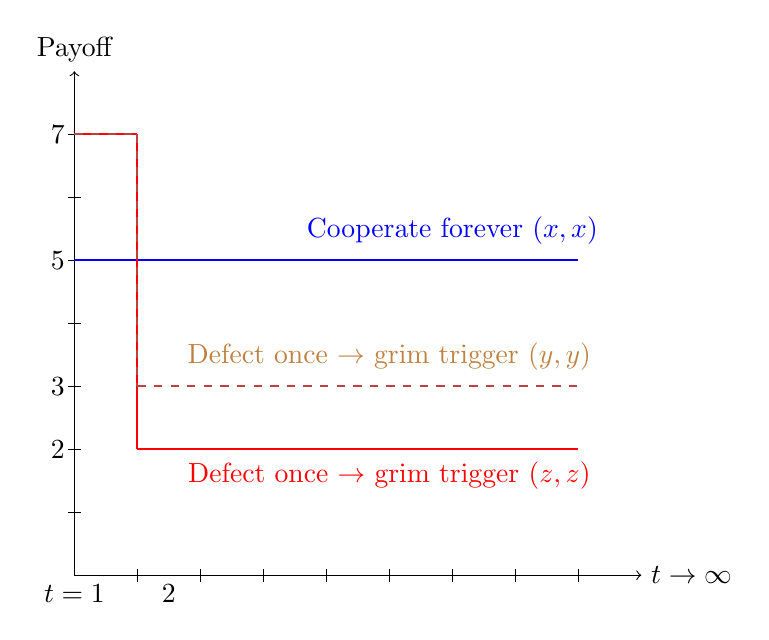
\begin{tikzpicture}[scale=0.8]
    % Axes
    \draw[->] (0,0) -- (9,0) node[right] {$t\rightarrow\infty$};
    \draw[->] (0,0) -- (0,8) node[above] {Payoff};
    % Ticks
    \foreach \x in {1,2,3,4,5,6,7,8}
      \draw (\x,0.1) -- (\x,-0.1);
    \foreach \y in {1,2,3,4,5,6,7}
      \draw (0.1,\y) -- (-0.1,\y);
    % Labels
    \node[left] at (0,5) {$5$};
    \node[left] at (0,2) {$2$};
    \node[left] at (0,3) {$3$};
    \node[left] at (0,7) {$7$};
    % --- Cooperate forever: constant at 5 ---
    \draw[thick, blue] (0,5) -- (8,5);
    \node[blue, above] at (6,5.1) {Cooperate forever $(x,x)$};
    % --- Defect once then harsh punishment z: 7 then 2 ---
    \draw[thick, red] (0,7) -- (1,7);
    \draw[thick, red] (1,7) -- (1,2);
    \draw[thick, red] (1,2) -- (8,2);
    \node[red, above] at (5,1.2) {Defect once $\rightarrow$ grim trigger $(z,z)$};
    % --- Defect once then soft punishment y: 7 then 3 ---
    \draw[thick, dashed, red!50!gray] (0,7) -- (1,7);
    \draw[thick, dashed, red!50!gray] (1,7) -- (1,3);
    \draw[thick, dashed, red!50!gray] (1,3) -- (8,3);
    \node[orange!50!gray, above] at (5,3.1) {Defect once $\rightarrow$ grim trigger $(y,y)$};
    % Period labels
    \node[below] at (0,0) {$t=1$};
    \node[below] at (1.5,0) {2};
    \end{tikzpicture}
    % \caption{Payoff paths under cooperation and grim-trigger punishments at $(z,z)$ and $(y,y)$}
    \end{figure}
\end{frame}

\begin{frame}{Grim Trigger with harsher punishment}
  Harsher punishments make cooperation easier to sustain:
  \begin{align*}
    \frac{5}{1-\delta} & \geq 7 + \frac{2\delta}{1-\delta} \\
    5 + \frac{5\delta}{1-\delta} & \geq 7 + \frac{2\delta}{1-\delta} \\
    \frac{(5-2)\delta}{1-\delta} & \geq 7-5 \\
    \delta & \geq \frac{2}{5}
  \end{align*}
\end{frame}

\begin{frame}{Tit-for-Tat}
  \underline{Player $i$} 
  \begin{align*}
    \begin{cases}
      t = 0 & \text{Play } x  \\ 
      t > 0 & \text{Play Player $j$'s strategy from } t-1 \\
    \end{cases} 
  \end{align*}

  \underline{Player $j$}
  \begin{itemize}
    \item In period $t=1$, cheat by playing $y$ to get payoff of 7
    \item In period $t>1$, go back to playing cooperatively
    \item $EV_{\text{Coop}} = 5 + 5\delta + \dots \frac{5}{1-\delta}$ 
    \item $EV_{\text{Cheat once}} = 7 + 2\delta + 5\delta^2 + 5\delta^3 + \dots = 7 + 2\delta + \frac{5\delta^2}{1-\delta}$
  \end{itemize}
\end{frame}

\begin{frame}{Tit-for-Tat}
  Solve for the value of $\delta$ for which this is a \textbf{SPNE}
  \begin{align*}
    5 + 5\delta + \frac{5\delta^2}{1-\delta} \geq & 7 + 2\delta + \frac{5\delta^2}{1-\delta} \\
    5 + 5\delta & \geq 7 + 2\delta \\
    \delta & \geq \frac{2}{3}
  \end{align*}
\end{frame}

\begin{frame}
  \begin{figure}[h]
    \centering
    \begin{tikzpicture}[scale=0.8]
    % Axes
    \draw[->] (0,0) -- (9,0) node[right] {$t\rightarrow\infty$};
    \draw[->] (0,0) -- (0,8) node[above] {Payoff};
    % Ticks
    \foreach \x in {1,2,3,4,5,6,7,8,9}
      \draw (\x,0.1) -- (\x,-0.1);
    \foreach \y in {1,2,3,4,5,6,7,8}
      \draw (0.1,\y) -- (-0.1,\y);
    % Labels
    \node[left] at (0,5) {$5$};
    \node[left] at (0,2) {$2$};
    \node[left] at (0,7) {$7$};
    % --- Cooperate forever: constant at 5 ---
    \draw[thick, blue] (0,5) -- (9,5);
    \node[blue, above] at (6,5.2) {Cooperate forever $(x,x)$};
    % --- Deviate once to y, then punished by z for one period, then forgiven ---
    \draw[thick, red] (0,7) -- (1,7);        % t=1 payoff = 7
    \draw[thick, red] (1,7) -- (1,3);        % drop to punishment
    \draw[thick, red] (1,3) -- (2,3);        % t=2 payoff = 3
    \draw[thick, red] (2,3) -- (2,5);        % forgiveness jump
    \draw[thick, red] (2,5) -- (9,5);        % back to cooperation
    \node[red, above] at (6,4.2) {Cheat once $y$ $\rightarrow$ TFT forgiveness};
    % Period labels
    \node[below] at (0,0) {$t=1$};
    \node[below] at (1.5,0) {2};
    \node[below] at (2.5,0) {3};
    \end{tikzpicture}
    % \caption{Payoff paths under cooperation and one-period-forgiveness Tit-for-Tat}
    \end{figure}
\end{frame}

\begin{frame}{A reciprocating cooperation strategy}
    \underline{Player $i$}
    $
      \begin{cases}
        t=0 & \text{Play } y \\ 
        t>0 & 
        \begin{cases}
          \text{Play } y \text{ if } t \text { is even } \\ 
          \text{Play } x \text{ if } t \text { is odd } \\ 
          \text{Play } z \text{ forever } 
          \text{ if P2 played } y 
          \text{ when $t$ is even} \\ 
        \end{cases}
      \end{cases} 
    $

    \underline{Player $j$}
    $
      \begin{cases}
        t=0 & \text{Play } x \\ 
        t>0 & 
        \begin{cases}
          \text{Play } y \text{ if } t \text { is odd } \\ 
          \text{Play } x \text{ if } t \text { is even } \\ 
          \text{Play } z \text{ forever } 
          \text{ if P2 played } y 
          \text{ when $t$ is odd} \\ 
        \end{cases}
      \end{cases} 
      $
\end{frame}

\begin{frame}{SPNE with reciprocation}
  What if Player $j$ defects in period 1?
  \begin{itemize}
    \item $EV_2(\text{Defect}) = 3 + 2\delta + 2\delta^2 + \dots = 3 + \frac{2\delta}{1-\delta}$
    \item $EV_2(\text{Coop}) = 2 + 7\delta + 2 \delta^2 + \dots = \frac{2+7\delta}{1-\delta^2}$
  \end{itemize}
  \begin{align*}
    \frac{2+7\delta}{1-\delta^2} & \geq 3 + \frac{2\delta}{1-\delta} \\
    \dots & \dots \\
    \delta^2 + 5\delta - 1 & \geq 0 \\
    \delta & > \approx 0.65 \\
  \end{align*}
\end{frame}

\begin{frame}{When can cooperation be achieved?}
  With all of these different ways of achieving repeated cooperation, 
  you might be wondering if there is a way to tell what strategies can actually work
  \begin{itemize}
    \item Punishment outcome must be BR in stage game
    \item Punishment strategies can't be exploitable (only credible threats)
    \item Different coordinating strategies are sustainable for different discount factors
  \end{itemize}
\end{frame}

\begin{frame}{Folk Theorem}
  Any strategy is a potential SPNE for a \textbf{repeated} stage game if: 
  \begin{itemize}
    \item Both agents are sufficiently patient and far-sighted (high enough $\delta$)
    \item The payoffs from the cooperative strategy profile satisfy the two properties: 
    \begin{itemize}
      \item \textbf{Individually Rational:} the payoffs to each agent (weakly) exceed their minimax payoffs in the stage game 
      \item \textbf{Feasibility:} the payoffs are weighted averages of the payoffs found in the stage game
    \end{itemize}
  \end{itemize}
\end{frame}

\begin{frame}{Folk Theorem with 3x3 Repeated Game Example}
  \begin{center}
  \begin{tabular}{*{5}{c|}}
  	\multicolumn{2}{c}{} & \multicolumn{3}{c}{Player $j$}\\ \cline{3-5}
    \multicolumn{1}{c}{} &       & x    & y    & z    \\\cline{2-5}
    \multirow{3}*{Player $i$}  & x & 5, 5 & 2, \underline{7} & 1, 3 \\\cline{2-5}
                             & y & \underline{7}, 2 & \underline{3}, \underline{3} & 0, 1 \\\cline{2-5}
                             & z & 3, 1 & 1, 0 & \underline{2}, \underline{2} \\\cline{2-5}
  \end{tabular}
  \end{center}
  The \alert{Minimax} equilibrium is (z,z)
  \begin{itemize}
    \item it \textit{minimizes} the \textit{maximum} payoff that your opponent could get
    \item The Minimax payoffs in this stage game are (2, 2)
    \item Intuitively, this is the \textit{safe} option: you can always fall back on it if cooperation fails
  \end{itemize}
\end{frame}

\begin{frame}{Incentive Compatible and Individually Rational conditions in 3x3 repeated game}
  \begin{figure}[!h]
  \centering
  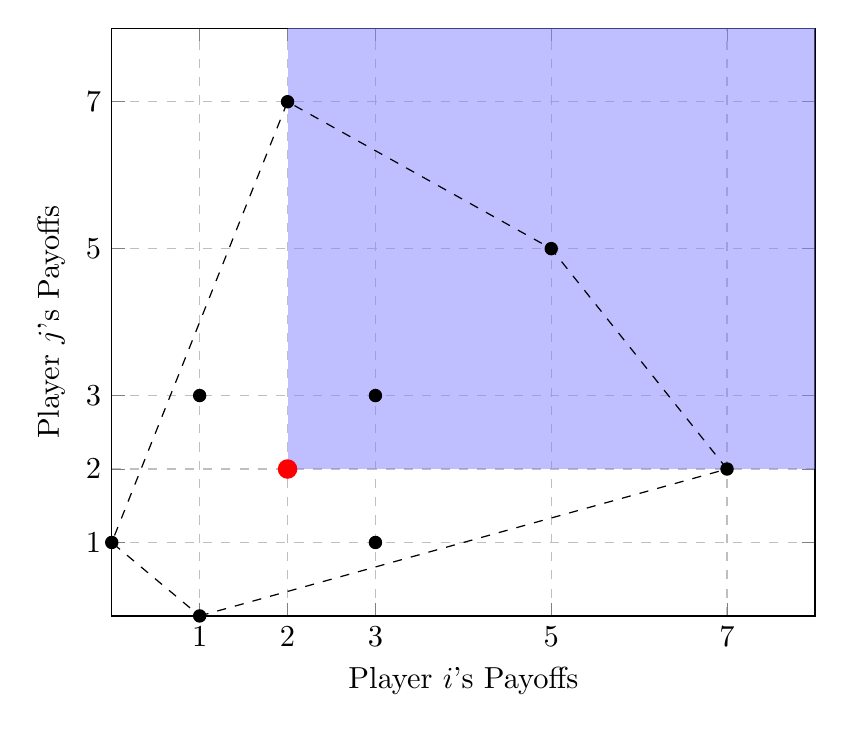
\begin{tikzpicture}[scale=1.1]
  \begin{axis}[
    width=0.8\textwidth,
    grid,
    xlabel={Player $i$'s Payoffs},
    ylabel={Player $j$'s Payoffs},
    xmin=0, xmax=8,
    ymin=0, ymax=8,
    xtick={1,2,3,5,7},
    ytick={1,2,3,5,7},
    grid style=dashed,
    legend style={at={(0.03,0.97)},anchor=north west},
  ]
  % --- Shaded Pareto-dominant region relative to (2,2) ---
  \addplot[
    fill=blue!50,
    fill opacity=0.5,
    draw=none
  ] coordinates {
    (2,2)
    (8,2)
    (8,8)
    (2,8)
  } -- cycle;
  % \addlegendentry{Pareto-dominates $(2,2)$}
  % --- Outline of the convex hull
  \addplot[
    dashed
  ] coordinates{
    (1,0)
    (7,2)
    (5,5)
    (2,7)
    (0,1)
  } --cycle;
  % --- Plot all payoff points ---
  \addplot[only marks]
  coordinates {
  (5,5) (2,7) (1,3) 
  (7,2) (3,3) (0,1)
  (3,1) (1,0) (2,2)
  };
  % \addlegendentry{Stage-game payoffs}
  % --- Highlight the minimax point (2,2) ---
  \addplot[
    only marks,
    mark=*,
    mark size=3,
    color=red
  ] coordinates {(2,2)};
  % \addlegendentry{Minimax $(2,2)$}
  \end{axis}
  \end{tikzpicture}
\end{figure}
\end{frame}

\begin{frame}{Folk Theorem with 3x3 Repeated Game Example}
  \begin{itemize}
    \item The shaded region of the graph shows us all of the strategy profiles which could be sustained by the \textbf{Folk Theorem} 
    \item This shows us why that strategy profile of alternating between (x, y) and (y, x) worked: 
    \begin{itemize}
      \item even though getting 2 on even or odd periods was no better than the Minimax payoffs, because you could alternate with the higher payoff of 7 you could do better as long as you are patient enough 
      \item this mix between (2, 7) and (7, 2) is \textit{within the convex hull} of feasible payoffs
    \end{itemize}
  \end{itemize} 
\end{frame}

% \begin{frame}{Cooperation in Repeated Games}
%   \begin{itemize}
%     \item As you can probably tell, there are an infinite number of strategy profiles which can achieve cooperation 
%     \begin{itemize}
%       \item We could allow for mixed strategies, which would work similar to the alternating example we saw 
%       \item The Folk Theorem tells us that all we need is for all players to be patient enough 
%       \item and also that the past plays are common knowledge
%     \end{itemize}
%   \end{itemize}
% \end{frame}

\begin{frame}{Importance of the Folk Theorem}
  Why does this matter for real life? 
  \begin{itemize}
    \item Most strategic interactions in your life are repeated 
    \item Even when you don't repeatedly interact with the same exact people, you still see cooperative outcomes 
    \item \textbf{Institutions, Reputations, and Social Structures} all serve to allow for past interactions to be common knowledge
    \item The history of humanity is built on how we arrange our strategic interactions in ways so that people are incentivized to play nice with others
  \end{itemize}
\end{frame}

\begin{frame}{Importance of the Folk Theorem}
  Some caveats:
  \begin{itemize}
    \item People can't know exactly when the game will end
    \begin{itemize}
      \item Institutions have to \textit{seem} like they are infinitely lived (compared to finitely lived humans)
    \end{itemize}
    \item Cooperative equilibria must beat outside options 
    \begin{itemize}
      \item If you make your institution too costly for people to engage with, they will opt out 
    \end{itemize}
    \item People need to be patient enough 
    \item Punishments must be credible
  \end{itemize}
\end{frame}


\end{document}
